\section{AlexNet}
2012'de ImageNet ILSVRC (Büyük Ölçekli Görsel Tanıma Yarışması)'de sunuldu. Alex Krizhevsky, Ilya Sutskever ve Geoffrey Hinton tarafından geliştirilmiştir. 5 convolutional ve 3 tane fully-connected katmandan oluşur. Aktivasyon olarak ReLU kullanır. İki paralel ağ şeklinde çalışır. AlexNet'in önceki CNN türlerinden farkı;

\begin{itemize}
    \item ReLU, önceki modellerde kullanılan tanh fonksiyonundan daha hızlı olduğundan eğitim süresini azaltmak için kullanılmıştır. Ayrıca ReLU etkinliğini sınırlamak için Local Response Normalization kullanılmıştır.
    \item Ezberlemeyi önlemek için seyreltme teknikleri uygulanmıştır.
    \item Eğitim setine “augmentation” işlemi uygulanmıştır. RGB kanallarının yoğunluklarını değiştirmek için PCA uygulamışlardır
\end{itemize}

\begin{figure}[h]
    \centering
    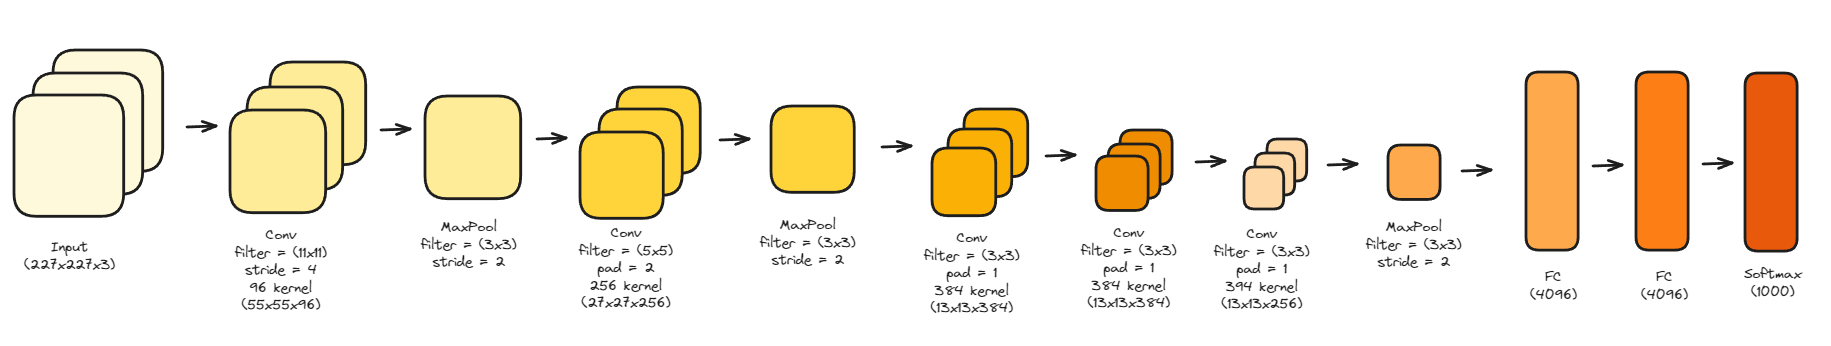
\includegraphics[width=1\textwidth]{images/alexnet.png}
    \caption{AlexNet mimarisi.}
    \label{fig:enter-label}
\end{figure}

\subsection{Mimarisi}
\begin{lstlisting}[language=Python]
model = Sequential([
	# (227-11) / 4 + 1 = 55 -> 55x55x96
	Conv2D(96, kernel_size=(11, 11), strides=4, padding="valid", activation="relu", input_shape=input_shape),
	# (55-3) / 2 + 1 = 27
	MaxPooling2D(pool_size=(3, 3), strides=(2, 2), padding="valid", data_format=None)

	# (27 + 2 * 2 - 5) / 1 + 1 = 27
	Conv2D(256, kernel_size=(5, 5), strides=1, padding="same", activation="relu", kernel_initializer="he_normal")
	# (27 - 3) / 2 + 1 = 13
	MaxPooling2D(pool_size=(3, 3), strides=(2, 2), padding="valid", data_format=None)

	# (13 + 2 * 1 - 3) / 1 + 1 = 13
	Conv2D(384, kernel_size=(3, 3), strides=1, padding="same", activation="relu", kernel_initializer="he_normal")
	# (13 + 2 * 1 - 3) / 1 + 1 = 13
	Conv2D(384, kernel_size=(3, 3), strides=1, padding="same", activation="relu", kernel_initializer="he_normal")
	# (13 + 2 * 1 - 3) / 1 + 1 = 13
	Conv2D(256, kernel_size=(3, 3), strides=1, padding="same", activation="relu", kernel_initializer="he_normal")

	# (13 - 3) / 2 + 1 = 6
	MaxPooling2D(pool_size=(3, 3), strides=(2, 2), padding="valid", data_format=None)

	# 4096
	Flatten(),

	Dense(4096, activation="relu")
	Dense(4096, activation="relu")
	Dense(1000, activation="relu")
	Dense(num_classes, activation="softmax")
])
\end{lstlisting}

\newpage